
%\section{Auswertung}


\section{Die Messwerte}
\begin{table}[H]
    \centering
    %\caption{Die Messwerte}
    \label{tab:messung}
    \begin{tabular}{ S [table-format=2.0] S [table-format=2.1] S[table-format=2.2] S S[table-format=2.1] S [table-format=3.0] }
        \toprule
        {$t \mathbin{/} \si{\minute}$} & {$T_1 \mathbin{/} \si{\celsius}$} & {${p^{*}}_1 \mathbin{/} \si{\bar}$} & 
        {$T_2 \mathbin{/} \si{\celsius}$} & {${p^{*}}_2 \mathbin{/} \si{\bar}$} & {$\symup{N} \mathbin{/} \si{\watt}$}\\
        \midrule
        0	& 21.7&	4.0 &	21.7  &  4.1 &   120\\
        0	& 21.7&	4.0 &	21.7  &  4.1&    120\\
        0	& 21.7&	4.0 &	21.7  &  4.1 &   120\\
        3 &	 25.3&	6.0 &	21.5&	3.5&	   120\\
        4 &	 26.4&	6.0 &	20.8&	3.5	&   120\\
        5 &	 27.5&	6.0 &	20.1&	3.4	&   120\\
        6 &	 28.8&	6.5 &	19.2&	3.3	 &  120\\
        7 &	 29.7&	6.5 &	18.5&	3.2	 &  120\\
        8 &	 30.9&	7.0 &	17.7&	3.2	 &  120\\
        9 	& 31.9&	7.0 &	16.9&	3.0	 &  120\\
        10	 &32.9&	7.0 &	16.2&	3.0	 &  120\\
        11	& 33.9&	7.5 &	15.5&	2.9  &   120\\
        12	& 34.8&	7.5 &	14.9&	2.8  &  120\\
        13	& 35.7&	8.0 &	14.2&	2.8 &	120\\
        14	 &36.7&	8.0 &	13.6&	2.7	  &  120\\
        15&	 37.6&	8.0 &	13.0&	2.6	 &   120\\
        16&	 38.4&	8.5 &	12.4&	2.6 &	120\\
        17&	 39.2& 8.5 &	11.7&	2.6	&    120\\
        18&	 40.0&	9.0 &	11.3&	2.5  &   120\\
        19&	 40.7&	9.0 &	10.9&	2.5	 &   120\\
        20&	 41.4&	9.0 &	10.4&	2.4	 &   120\\
        21&	 42.2&	9.0 &	9.9	 &   2.4	 &   120\\
        22&	 42.9&	9.5 &	9.5	&    2.4	 &   120\\
        23&	 43.6&	9.5 &	9.1	&    2.4	 &   120\\
        24&	 44.3&	10.0&	8.7&    2.4	&    120\\
        25&	 44.9&	10.0&	8.3	&    2.4	 &   120\\
        26&	 45.5&	10.0&	8.0&	    2.3	 &   120\\
        27&	 46.1&	10.0&	7.7	&    2.2	 &   122\\
        28&	 46.7&	10.5&	7.4&	    2.2	 &   122\\
        29&	 47.3&	10.5&	7.1&	    2.2	 &   122\\
        30&	 47.8	&10.75&	6.8	&    2.2	 &   122\\
        31&	 48.4&	11.0&	5.6	 &   2.2	&    122\\
        32&	 48.9&	11.0&	4.3	&    2.2	 &   122\\
        33&	 49.4&	11.0&	3.4	&    2.2	 &   122\\
        34&	 49.9&	11.0&	3.0	&    2.2	&    122\\
        35&	 50.3&	11.0&	2.9	&    2.2	 &   122\\
        \bottomrule
        %\multicolumn{6}{c}{$\text{Eine Tabelle der Messwerte,}$}
        %\multicolumn{6}{c}{$\text{wobei die Temperaturen mit einem Fehler von  $\increment T = \SI{0.1}{\celsius}$ behaftet sind.}$}
    \end{tabular}
\caption{Eine Tabelle der Messwerte, wobei die Temperaturen mit einem Fehler von  $\increment T = \SI{0.1}{\celsius}$ behaftet sind.}
\end{table}

\FloatBarrier
\section{Auswertung}
%5a)
\subsection{Gefitete Messwerte}
\subsubsection{Plot der Messwerte und Funktionen}
\begin{figure}
    \centering
    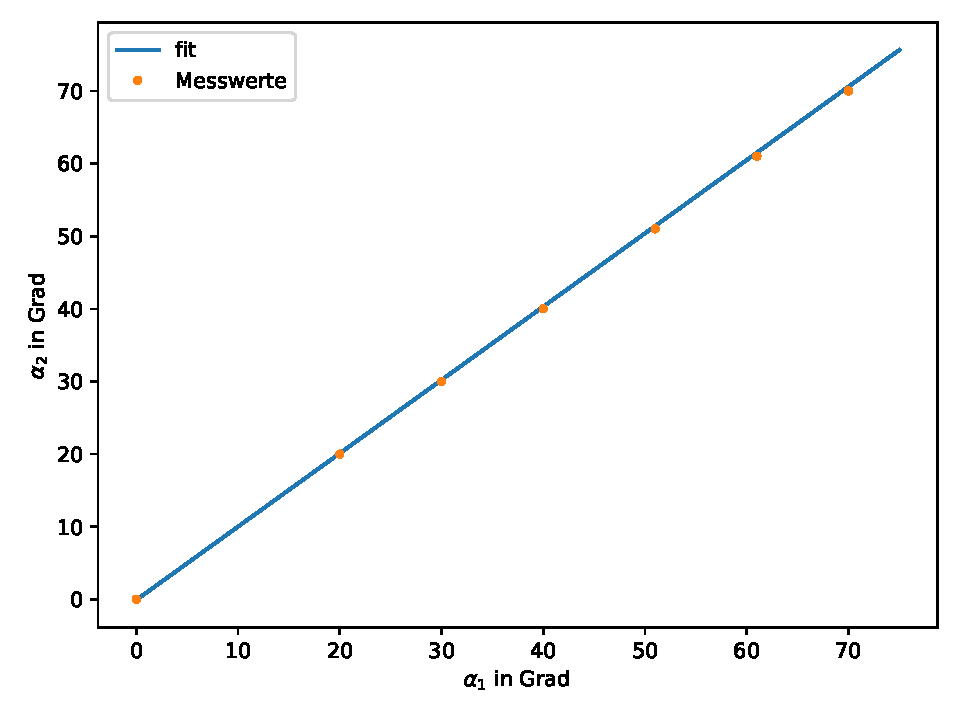
\includegraphics[width=0.85\textwidth]{build/plot1.pdf}
    \caption{Ein Plot der Messwerte inklusive der gefiteten Funktionen.}
    \label{img:plot1}
\end{figure}


%5b)
\subsubsection{Fit-Funktionen}
Dies sind die Fit-Funktionen auf die Messwerte. Dabei ist der Fit auf $T_1$ die Funktion $F(t)$ und der auf $T_2$ ist die Funktion $G(t)$.
\begin{align}
    &F(t) =A \cdot t^2+B \cdot t+ C \\
    &G(t) = \frac{D}{1+E \cdot t^{F}}\\ 
    \nonumber
    \\
    &\begin{aligned}
        A &=(-3.22\pm 0.04)\cdot 10^{-6} & B&=0.02028\pm 0.00009 & C&=294.97\pm 0.04 \\
        D &=296.0\pm 0.4 & E&= (6.3\pm 2.1)\cdot 10^{-5}& F&=0.92\pm 0.04
    \end{aligned}\\
    \nonumber
    \\
    \implies &F(t) =(-3.22\pm 0.04)\cdot 10^{-6}\cdot t^2+(0.02028\pm 0.00009)t+294.97\pm 0.04 \\
    \implies &G(t) = \frac{296.0\pm 0.4}{1+(6.3\pm 2.1)\cdot 10^{-5}\cdot t^{0.92\pm 0.04}}
\end{align}
\\
%5c)
\subsection{Differentialquotienten der Temperaturen}
Im folgenden werden die Differentialquotienten der Temperaturen in verschiedenen Stellen berechnet.
Da die Fit Funktionen eine angemessene Abbildung der Messwerte darstellen berechnen wir die Quotienten über das bilden der Ableitung der Fits $F(t)$ und $G(t)$ 
und ihrer anschließenden Punktweisen Auswertung.
Als Punkte wurden hierbei 7er Schritte gewählt, da man daurch regelmäßige Abstände über den Definitonsbereich hat und einen breiten Bereich des selben abdeckt.


\begin{align}
    \frac{\partial F(t)}{\partial t} &=2At*B & \frac{\partial G(t)}{\partial t} &= \frac{-D \cdot F\cdot E \cdot t^{F-1}}{(1+E\cdot t^{F})^{2}}
\end{align}

\begin{table}[H]
    \centering
    \begin{tabular}{S[table-format=2.0] S [table-format=3.5] @{$\pm{}$} S  S [table-format=3.5] @{$\pm{}$} S}
        \toprule
        {Zeit [min]} & \multicolumn{2}{c}{ $\frac{\partial F(t)}{\partial t} \mathbin{\scalebox{1.5}{/}} \si{\kelvin\per\second}$ } & \multicolumn{2}{c}{ $\frac{\partial G(t)}{\partial t} \mathbin{\scalebox{1.5}{/}} \si{\kelvin\per\second}$ }  \\
        \midrule
        7  & -0.0172 & 0.0001 &  0.0100& 0.0077\\
        14 & -0.0145 & 0.0002 &  0.0093& 0.0072\\
        21 & -0.0118 & 0.0002 &  0.0087& 0.0067\\
        28 & -0.0091 & 0.0002 &  0.0083& 0.0062\\ 
        \bottomrule      
    \end{tabular}
\caption {Werte der Zeittlichen Ableitungen der Temperaturen.}
\label{tab:Diff}
\end{table}

%5d)
\subsection{Güteziffern}
Anschließend werden die idealen und realen Güteziffern der Wärmepumpe aus den zuvor berechneten Werten und 
den Formeln \eqref{eqn:videal} und \eqref{eqn:vreal}  bestimmt. 
Dabei werden für die Temperaturwerte immer für verschiedene Zeiten die korrespondierenden Messwerte genutzt.

\begin{equation}
    v_\text{ideal}= \frac{Q_1}{A} = \frac{T_1}{T_1-T_2}
    \label{eqn:videal}
\end{equation}

\begin{equation}
    v_\text{real}= \frac{\increment{Q_1}}{\increment t \cdot \symup{N} }
    \label{eqn:vreal}
\end{equation}

\begin{equation}
    \frac{\increment Q_1}{\increment t} = \left(m_1 c_w + m_k c_k \right)\frac{\increment T_1}{\increment t}
    \label{eqn:delQ1}
\end{equation}
\\
Für die reale Wärmepumpe gilt $v_\text{real} < v_\text{ideal}$.\\
\\
Der Wert für die reale Wärmepumpe lässt sich dann bestimmen, 
in dem man für die Wärmekapazität der Kupferschlange $m_k c_k =\SI{750}{\joule\per\kelvin}$,
für die Masse des Wassers $m_1=\SI{4}{\kilo\gram}$ und für die spezifische Wärmekapazität 
des Wassers $c_w=\SI{4.183}{\kilo\joule\per\kilo\gram\per\kelvin}$ \footnote[3]{Quelle: \url{https://www.chemie.de/lexikon/Spezifische_W\%C3\%A4rmekapazit\%C3\%A4t.html}
(Besucht am 30.11.2020)} nimmt.
Anschließend setzt man dann \eqref{eqn:delQ1} in \eqref{eqn:vreal} ein.\\
Es ergibt sich dann also aus den genannten Werten und den Werten aus \ref{tab:Diff} ;
\begin{table}[H]
    \centering
    
    \begin{tabular}{ S [table-format=2.0] S [table-format=1.5] S [table-format=1.5] }
        \toprule
        {$t \mathbin{/} \si{\minute}$} & { $v_\text{ideal}$} & {$v_\text{real} $} \\
        \midrule
        7	& 31.4375  & 0.12929\\
        14	& 14.35814 & 0.12900\\
        21	& 10.14194 & 0.12871\\
        28	& 8.3099   & 0.12632\\
        \bottomrule
        \\
    \end{tabular}
\caption {Berechnete Werte für $v_\text{ideal}$ und $v_\text{real} $ gerundet auf die fünfte Nachkommastelle.}
\label{tab:vreal}
\end{table}


Wie man sieht sind die realen Güteziffer sogar teilweise um einen Faktor $10^3$ kleiner als die der idealen Güteziffer.
Dafür unterliegen sie wesentlich weniger Fluktuationen. Man sieht, dass sie ungefähr einen Wert von $\approx 0.129$haben, 
wobei die Werte von $v_\text{ideal}$ so sehr schwanken, dass sich keine vernünftige Abschätzung machen lässt.
\newpage
%5e)
\subsection{Massendurchsatz}
\subsubsection{Plot und Verdampfungswärme}

\begin{figure}
    \centering
    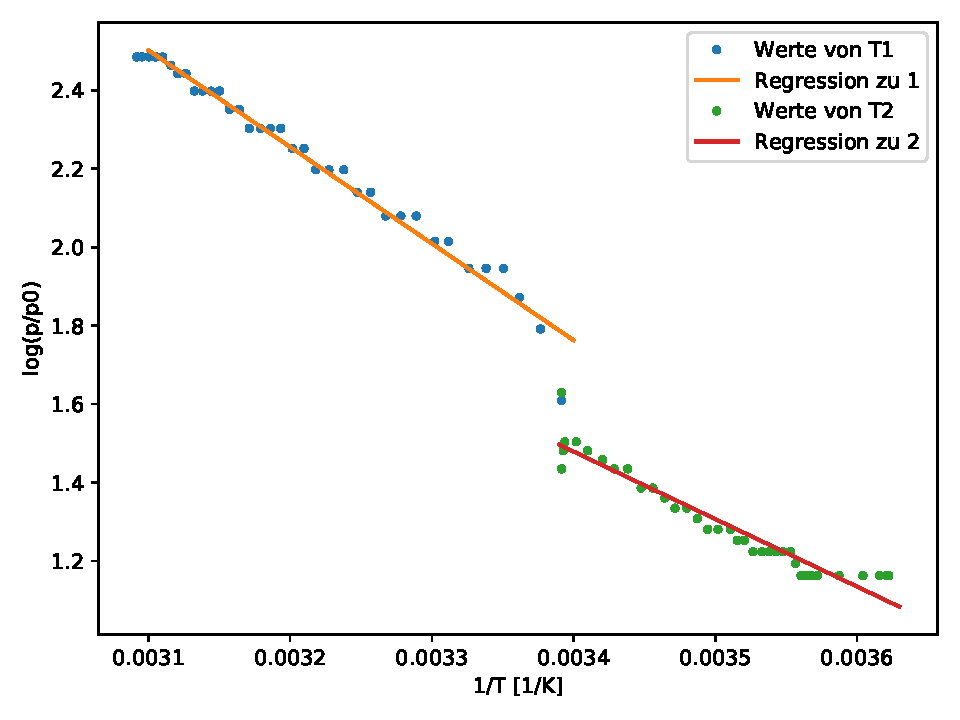
\includegraphics[width=\textwidth]{build/plot2.pdf}
    \caption{Druck-Temperatur Abbildung mit Ausgleichsgerade zur Bestimmung der Verdampfungswärme $L$.}
\end{figure}

Mithilfe einer linearen Regression lässt sich nun aus den geploteten Werten 
die Verdampfungswärme $L$ von Dichloridfluormethan $\ce{Cl2F2C}$ bestimmen.
\footnotetext[4]{Quelle: \url{https://www.chemie.de/lexikon/Universelle_Gaskonstante.html}(Besucht am 30.12.2020)}


\begin{align*}
\intertext{$L$ bestimmt sich dann aus der Regressionsgeraden des Datensatzes $T_2$
 mit Hilfe der Gaskonstante $\symup{R}$ \footnotemark[2].}
\\
\implies L&=(-1) \cdot m \cdot \symup{R}\\
y&=-1718.02083898x+7.3235009\\
\\
\implies L&\approx\SI{14298.66+-734.7}{\joule\per\mol}
\intertext{Die Verdampfungswärme läst sich nun mithilfe der Molaren Masse von \si{Joule\per\mol} zu \si{\joule\per\kilogramm} umrechnen.}
m_{\text{molar}}&=\SI{120.91 e-3}{\kilogram\per\mol} \footnotemark[5]
\implies L&\approx\SI{118258.7336+-6076.4305}{\joule\per\kilogram} 
\end{align*}
\footnotetext[5]{Quelle: \url{https://www.chemie.de/lexikon/Dichlordifluormethan.html}(Besucht am 30.12.2020)}
%\footnotetext[2]{Quelle: \url{https://www.chemie.de/lexikon/Universelle_Gaskonstante.html}(Besucht am 30.11.2020)}



\subsubsection{Berechnung Massendurchsatz}

Nun lässt sich Mithilfe der Verdampfungswärme von Dichloridfluormethan und der Formel \refeq{eqn:mass} und \refeq{eqn:delQ2} der Massendurchsatz bestimmen.
Dafür werden wieder die Werte, die für \refeq{eqn:delQ1} genutzt wurden, mit $m_2= m_1= \SI{4}{\kilo\gram}$, genutzt.
\begin{equation}
    \frac{\increment Q_2}{\increment t} = \left(m_2 c_w + m_k c_k \right)\frac{\increment T_2}{\increment t}
    \label{eqn:delQ2}
\end{equation}
\begin{equation}
    \frac{\increment Q_2}{\increment t} = L\cdot \frac{\increment m}{\increment t}
    \label{eqn:mass}
\end{equation}

Einsetzen in diese Formel führt zu:
\begin{table}[H]
    \centering
    \begin{tabular}{ S [table-format=1.5] S [table-format=1.5] @{$\pm{}$} S}
        \toprule
        {$t \mathbin{/} \si{\minute}$} & \multicolumn{2}{c}{ $\frac{\Delta m}{\Delta t} \mathbin{\scalebox{1.5}{/}} \si{\kilo\gram\per\second}$}\\
        \midrule
        7	&-0.01225  & 0.00066\\
        14	&-0.01131  & 0.00061\\
        21	&-0.01068  & 0.00058\\
        28	&-0.01018  & 0.00055\\
        \bottomrule
        \\
    \end{tabular}
\caption {Berechnete Werte für den Massendurchsatz $m$ von $\ce{Cl2F2C}$ gerundet auf die fünfte Nachkommastelle.}
\label{tab:mass}
\end{table}


\subsection{Kompressorleistung}
\begin{align*}
 %   \intertext{Die Kompressorleistung ergibt sich als die Kompressionsarbeit pro Zeit, also als:}
%    N_\text{mech}&=\frac{\increment A_m}{\increment t}
 %   \intertext{Des Weiteren ist die Kompressionsarbeit die Arbeit, welche verrichtet wird, wenn ein Stoff eines Volumens zu einem anderen Volumen komprimiert wird.}
%    A_m&= - \int_{V_a}^{V_b} p \, \symup{d}V
%    \intertext{Für die Berechnung der Kompressorleistung  $N_\text{mech}$ darf eine adiabatische Kompression angenommen wertden, 
%    weswegen die Poissonsche Gelichung genutzt werden kann.}
%    p_a V_a^{\kappa} &= p_a V_a^{\kappa} =p V^{\kappa}
 %   \intertext{Wobei $\kappa$ das Verhältinis der molwärmen der beiden [Dunno] ist und als $\kappa =1.14 $ gegeben ist.
    \intertext{Mit Hilfe der in \ref{kompressor} hergeleiteten Formel lässt sich nun die Kompressorleistung bestimmen.}
   \intertext{Dabei sind $\kappa =1.14 $, $p=\SI{1}{\bar}$, $T=\SI{0}{\celsius}$ und $\rho_0=\SI{5.51}{\gram\per\litre}$ als die Werte gegeben.}
   \intertext{Und die Formel die sich zur Bestimmung ergeben hat:}
   N_\text{mech} &= \frac{1}{\kappa-1}\left( p_b \sqrt[\kappa]{\frac{p_a}{p_b}}-p_a \right) \frac{1}{\rho} \frac{\increment m}{\increment t}
\end{align*}
Wieder mit den Werten aus \ref{tab:Diff} lässt sich so die Leistung bestimmen.
\begin{table}[H]
    \centering
    \begin{tabular}{ S [table-format=2.0] S [table-format=1.5] @{$\pm{}$} S[table-format=1.4]}
        \toprule
        {$t \mathbin{/} \si{\minute}$} & \multicolumn{2}{c}{ $P \mathbin{/} \si{\watt}$} \\
        \midrule
        7	&-0.0055& 0.0003\\
        14	&-0.0063& 0.0003\\
        21	&-0.0070& 0.0004\\
        28	&-0.0072& 0.0004\\
        \bottomrule
        \\
    \end{tabular}
    \caption{Die berechneten Werte von $N_\text{mech}$ in $\si{\watt}$ gerundet auf die vierte Nachkommastelle. }
    \label{tab:leistung}
\end{table}

%5g)
\subsection{Fazit zur Güteziffer} \label{fazit}

Die große Diskrepanz zwischen idealer und realer Güteziffer, die man in \ref{tab:vreal} und \ref{eqn:videal} sieht,
läasst sich vermutlich dadurch erklären, dass in dem Vorgang sehr viel Energie in bei der Umwandlung
"verloren" geht.
Zu diesen Prozessen gehören zum Beispiel die Pumpen, bei denen in durch Reibung viel Energieverluste entstehen
oder durch den mechanischen Transport der Kühlflüssigkeit, die viel Energie benötigt.
Diese Energieverluste lassen sich auch mit großem Aufwand schlecht minimieren, weswegen dort eine große Diskrepanz entsteht.



%Dichloridfluormethan $\ce{Cl2F2C}$
%\begin{align*}
%\intertext{Es ergibt sich dann also;}V
%\end{align*}

